% Source-faithful schematic draft: 2005 Beijing Arts Q20, PDF p.2 (printed p.219).
% Source ID: src-fea4e73708ac3a85394b3698456c3244904a156c2ea4907c94a9bc9ed3e6cf8d
% Source SHA-256: 9ee1bf91b64cd5e48bd6415909f82ef61e023a117a843043c0ca22435102b3a1
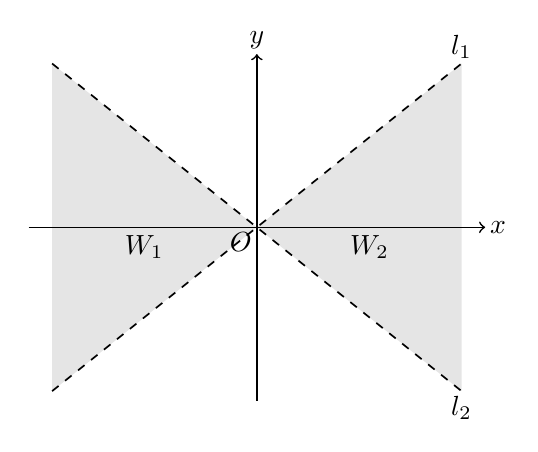
\begin{tikzpicture}[line width=0.6pt, scale=1.0, every node/.style={inner sep=1.5pt}, baseline=(current bounding box.center)]
  % Axes limits
  \def\xmax{2.6}
  \def\ymax{2.0}
  \def\k{0.8}

  % Shaded regions W1 and W2
  \fill[gray!20] (-\xmax, {-\k*\xmax}) -- (0, 0) -- (-\xmax, {\k*\xmax}) -- cycle;
  \fill[gray!20] (\xmax, {-\k*\xmax}) -- (0, 0) -- (\xmax, {\k*\xmax}) -- cycle;

  % Boundary dashed lines l1 and l2
  \draw[dashed, line width=0.6pt] (-\xmax, {-\k*\xmax}) -- (\xmax, {\k*\xmax}) node[above] {$l_1$};
  \draw[dashed, line width=0.6pt] (-\xmax, {\k*\xmax}) -- (\xmax, {-\k*\xmax}) node[below] {$l_2$};

  % Solid coordinate axes
  \draw[->] (-\xmax-0.3, 0) -- (\xmax+0.3, 0) node[right] {$x$};
  \draw[->] (0, -\ymax-0.2) -- (0, \ymax+0.2) node[above] {$y$};

  % Labels
  \node[below left] at (0, 0) {$O$};
  \node at ({-0.55*\xmax}, -0.25) {$W_1$};
  \node at ({0.55*\xmax}, -0.25) {$W_2$};
\end{tikzpicture}
